\documentclass[9pt]{beamer}
\usetheme{metropolis}
\usepackage{amsmath}
\usepackage{amssymb}
\usepackage{graphicx}
\usepackage{booktabs}
\usepackage{xcolor}
\usepackage{tikz}
\usetikzlibrary{arrows,positioning,shapes.geometric,calc}

% Define color palette matching our project design system
\definecolor{primary}{HTML}{1abc9c}    % Deep Teal
\definecolor{secondary}{HTML}{3498db}  % Astro Blue
\definecolor{darkbg}{HTML}{2c3e50}     % Slate Blue
\definecolor{accent}{HTML}{e67e22}     % Orange

\setbeamercolor{palette primary}{bg=darkbg, fg=white}
\setbeamercolor{palette secondary}{bg=primary, fg=white}
\setbeamercolor{palette tertiary}{bg=secondary, fg=white}
\setbeamercolor{structure}{fg=primary}
\setbeamercolor{alerted text}{fg=accent}

\title{Bayesian Statistics \& Markov Chain Monte Carlo (MCMC)}
\subtitle{A Comprehensive Tutorial: From Probability Foundations to Sampling Diagnostics}
\author{Astronomy Club}
\date{\today}

\begin{document}

\maketitle

% Slide 2: Table of Contents / Modules
\begin{frame}{Tutorial Roadmap}
  This tutorial teaches Bayesian inference and Markov Chain Monte Carlo (MCMC) starting from the absolute basics of probability theory, with no prior statistics background assumed:
  \begin{description}
    \item[Module 1:] \textbf{Foundations of Bayesian Inference}
      \begin{itemize}
        \item Frequentist vs. Bayesian probability, Bayes' Theorem, priors, likelihoods, posteriors, and the normalizing evidence challenge.
      \end{itemize}
    \item[Module 2:] \textbf{Markov Chains \& Monte Carlo Integration}
      \begin{itemize}
        \item Random sampling integration, properties of Markov chains, memorylessness, and stationary convergence.
      \end{itemize}
    \item[Module 3:] \textbf{The Metropolis-Hastings Algorithm}
      \begin{itemize}
        \item Bypassing normalizers, symmetric proposals, acceptance ratios, and the complete algorithm flowchart.
      \end{itemize}
    \item[Module 4:] \textbf{MCMC Diagnostics \& Best Practices}
      \begin{itemize}
        \item Burn-in phases, trace plots, autocorrelation, joint posterior corner plots, and proposal width tuning.
      \end{itemize}
  \end{description}
\end{frame}

% Module 1 Header
\begin{frame}[plain]
  \vfill
  \centering
  \begin{beamercolorbox}[sep=8pt,center,shadow=true,rounded=true]{palette primary}
    \usebeamerfont{title}\textbf{Module 1: Foundations of Bayesian Inference}
  \end{beamercolorbox}
  \vfill
\end{frame}

% Slide 4: Frequentist vs. Bayesian Probability
\begin{frame}{Frequentist vs. Bayesian Probability}
  To understand Bayesian statistics, we must first contrast how it defines ``probability'' compared to classical frequentist statistics:
  \begin{description}
    \item[Frequentist Probability (Objective Limit):]
      Probability is the limiting relative frequency of an event in an infinite sequence of identical, repeatable trials.
      \begin{itemize}
        \item \alert{Limitation:} Cannot assign a probability to one-off, non-repeatable events (e.g., ``What is the probability that the universe has a flat geometry?'' or ``What is the probability that this specific galaxy hosts a Type Ia supernova?'').
      \end{itemize}
    \item[Bayesian Probability (Degree of Belief):]
      Probability is a measure of our state of knowledge or degree of belief given incomplete information.
      \begin{itemize}
        \item \alert{Advantage:} Allows us to update our beliefs as new data arrives and to quantify uncertainties on constant physical parameters (like supernova rate coefficients $A$ and $B$).
      \end{itemize}
  \end{description}
\end{frame}

% Slide 5: Bayes' Theorem Derivation
\begin{frame}{Bayes' Theorem Derivation}
  Bayes' Theorem is the fundamental equation of Bayesian inference. We derive it directly from the definition of conditional probability:
  \begin{itemize}
    \item The joint probability of two events $A$ and $B$ occurring is:
      $$P(A \cap B) = P(A \mid B) \cdot P(B)$$
    \item By symmetry, we can also express this joint probability as:
      $$P(A \cap B) = P(B \mid A) \cdot P(A)$$
    \item Equating the two right-hand sides:
      $$P(A \mid B) \cdot P(B) = P(B \mid A) \cdot P(A)$$
    \item Dividing both sides by $P(B)$ yields Bayes' Theorem:
      $$P(A \mid B) = \frac{P(B \mid A) \cdot P(A)}{P(B)}$$
  \end{itemize}
\end{frame}

% Slide 6: The Components of Bayesian Parameter Inference
\begin{frame}{The Components of Bayesian Parameter Inference}
  In scientific parameter estimation, we replace event $A$ with our model parameters $\theta$ (e.g., rate coefficients $A, B$), and event $B$ with our observations $D$ (host galaxy catalog):
  $$P(\theta \mid D) = \frac{P(D \mid \theta) P(\theta)}{P(D)}$$
  \begin{description}
    \item[Posterior $P(\theta \mid D)$:] What we know about the parameters $\theta$ \textbf{after} seeing the data $D$. This is our target probability distribution.
    \item[Likelihood $P(D \mid \theta)$:] The probability of observing the data $D$ given a specific parameter set $\theta$.
    \item[Prior $P(\theta)$:] What we knew about the parameters $\theta$ \textbf{before} seeing the data $D$ (based on previous experiments or physical boundaries).
    \item[Evidence $P(D)$:] The normalizing marginal likelihood (a constant).
  \end{description}
\end{frame}

% Slide 7: The Normalization Challenge
\begin{frame}{The Normalization Challenge}
  To ensure the posterior is a valid probability distribution (integrates to $1.0$), we divide by the evidence $P(D)$. By the law of total probability, the evidence is the integral of the numerator over the entire parameter space:
  $$P(D) = \int_{\theta} P(D \mid \theta) P(\theta) d\theta$$
  \begin{alertblock}{The Curse of Dimensionality}
    If we have a single parameter $\theta$, this integral is easy to solve. If we have $d=10$ parameters, and we divide the parameter range into $100$ grid points, we must evaluate:
    $$100^{10} = 10^{20} \text{ likelihood calculations}$$
    which would take supercomputers years to calculate. For high-dimensional physical models, solving this integral analytically or via simple numerical integration is impossible.
  \end{alertblock}
\end{frame}

% Module 2 Header
\begin{frame}[plain]
  \vfill
  \centering
  \begin{beamercolorbox}[sep=8pt,center,shadow=true,rounded=true]{palette primary}
    \usebeamerfont{title}\textbf{Module 2: Markov Chains \& Monte Carlo Integration}
  \end{beamercolorbox}
  \vfill
\end{frame}

% Slide 9: What is Monte Carlo Integration?
\begin{frame}{What is Monte Carlo Integration?}
  If we cannot solve the normalization integral analytically, how do we evaluate the posterior? We use **Monte Carlo Integration** (sampling):
  \begin{itemize}
    \item Instead of evaluating an integral analytically, we draw random independent samples $\{\theta_1, \theta_2, \dots, \theta_M\}$ from the probability distribution.
    \item \textbf{Example: Estimating $\pi$ by throwing random darts:}
      \begin{enumerate}
        \item Draw a circle of radius $r$ inside a square of side $2r$.
        \item Generate random coordinates $(x, y)$ inside the square.
        \item Count the fraction of coordinates that fall inside the circle:
          $$\frac{N_{\text{inside}}}{N_{\text{total}}} \approx \frac{\text{Area}_{\text{circle}}}{\text{Area}_{\text{square}}} = \frac{\pi r^2}{4r^2} = \frac{\pi}{4} \implies \pi \approx 4 \cdot \frac{N_{\text{inside}}}{N_{\text{total}}}$$
      \end{enumerate}
    \item By drawing samples from the posterior, we can compute averages, standard deviations, and confidence intervals directly from the sample histograms without ever calculating the normalizer $P(D)$.
  \end{itemize}
\end{frame}

% Slide 10: What is a Markov Chain?
\begin{frame}{What is a Markov Chain?}
  How do we draw samples from a complex, non-standard posterior distribution $P(\theta \mid D)$? We construct a \textbf{Markov Chain}.
  \begin{block}{The Markov Property (Memorylessness)}
    A Markov Chain is a sequence of random variables $\{\theta_0, \theta_1, \theta_2, \dots, \theta_t\}$ where the probability of the next state $\theta_{t+1}$ depends \textbf{only} on the current state $\theta_t$, not on the history of previous states:
    $$P(\theta_{t+1} \mid \theta_0, \theta_1, \dots, \theta_t) = P(\theta_{t+1} \mid \theta_t)$$
  \end{block}
  \begin{itemize}
    \item We start at a random point in parameter space.
    \item At each step $t$, we propose a transition to a new state $\theta_{\text{prop}}$ based on a transition probability that depends only on $\theta_t$.
    \item If we design the transition rules correctly, the distribution of samples will converge to a unique \textbf{stationary distribution} that matches our target posterior $P(\theta \mid D)$.
  \end{itemize}
\end{frame}

% Module 3 Header
\begin{frame}[plain]
  \vfill
  \centering
  \begin{beamercolorbox}[sep=8pt,center,shadow=true,rounded=true]{palette primary}
    \usebeamerfont{title}\textbf{Module 3: The Metropolis-Hastings Algorithm}
  \end{beamercolorbox}
  \vfill
\end{frame}

% Slide 12: Bypassing the Normalizer: The Posterior Ratio
\begin{frame}{Bypassing the Normalizer: The Posterior Ratio}
  The core magic of Markov Chain Monte Carlo (MCMC) is that we do not need to calculate the evidence $P(D)$.
  \begin{itemize}
    \item When deciding whether to move from current state $\theta_t$ to proposed state $\theta_{\text{prop}}$, we compare their posterior probabilities as a ratio:
      $$\frac{P(\theta_{\text{prop}} \mid D)}{P(\theta_t \mid D)} = \frac{\left( \frac{P(D \mid \theta_{\text{prop}}) P(\theta_{\text{prop}})}{P(D)} \right)}{\left( \frac{P(D \mid \theta_t) P(\theta_t)}{P(D)} \right)} = \frac{P(D \mid \theta_{\text{prop}}) P(\theta_{\text{prop}})}{P(D \mid \theta_t) P(\theta_t)}$$
    \item Notice that the evidence constant $P(D)$ in the denominator cancels out!
    \item We only need to calculate the likelihoods and priors of the two states to determine the transition probability.
  \end{itemize}
\end{frame}

% Slide 13: Proposal Distributions and Acceptance
\begin{frame}{Proposal Distributions and Acceptance}
  How does the Metropolis-Hastings algorithm navigate the parameter space?
  \begin{itemize}
    \item \textbf{Proposal Distribution $q(\theta_{\text{prop}} \mid \theta_t)$:}
      A probability function used to suggest the next step. Typically a symmetric Gaussian centered on the current state:
      $$\theta_{\text{prop}} \sim \mathcal{N}(\theta_t, \sigma^2)$$
      Because it is symmetric, proposing $\theta_{\text{prop}}$ from $\theta_t$ has the same probability as proposing $\theta_t$ from $\theta_{\text{prop}}$: $q(\theta_{\text{prop}} \mid \theta_t) = q(\theta_t \mid \theta_{\text{prop}})$.
    \item \textbf{Acceptance Probability ($\alpha$):}
      The probability that we accept the proposed transition:
      $$\alpha = \min\left(1, \frac{P(D \mid \theta_{\text{prop}}) P(\theta_{\text{prop}})}{P(D \mid \theta_t) P(\theta_t)}\right)$$
      \begin{itemize}
        \item If the proposal increases the posterior, $\alpha = 1.0$ (we always accept).
        \item If the proposal decreases the posterior, $\alpha < 1.0$ (we might accept).
      \end{itemize}
  \end{itemize}
\end{frame}

% Slide 14: Step-by-Step Metropolis-Hastings Algorithm
\begin{frame}{Step-by-Step Metropolis-Hastings Algorithm}
  To run an MCMC chain:
  \begin{enumerate}
    \item **Initialize:** Choose a starting parameter point $\theta_0$ and a proposal step width $\sigma$.
    \item **Loop:** For each step $t$ from $0$ to $M-1$:
      \begin{itemize}
        \item Propose a candidate state: $\theta_{\text{prop}} \sim \mathcal{N}(\theta_t, \sigma^2)$.
        \item Evaluate prior boundaries. If $\theta_{\text{prop}}$ is unphysical (outside priors), reject: set $\theta_{t+1} = \theta_t$ and skip to next step.
        \item Calculate the acceptance probability:
          $$\alpha = \min\left(1, \frac{\text{Likelihood}(\theta_{\text{prop}}) \cdot \text{Prior}(\theta_{\text{prop}})}{\text{Likelihood}(\theta_t) \cdot \text{Prior}(\theta_t)}\right)$$
        \item Draw a random number $u \sim \mathcal{U}(0, 1)$.
        \item If $u < \alpha$:
          Accept proposal: set $\theta_{t+1} = \theta_{\text{prop}}$.
        \item Else:
          Reject proposal: set $\theta_{t+1} = \theta_t$.
      \end{itemize}
  \end{enumerate}
\end{frame}

% Slide 15: Metropolis-Hastings Decision Flowchart
\begin{frame}{Metropolis-Hastings Decision Flowchart}
  Below is the step-by-step decision pathway executed at each iteration of the Metropolis-Hastings MCMC sampler:
  \vfill
  \centering
  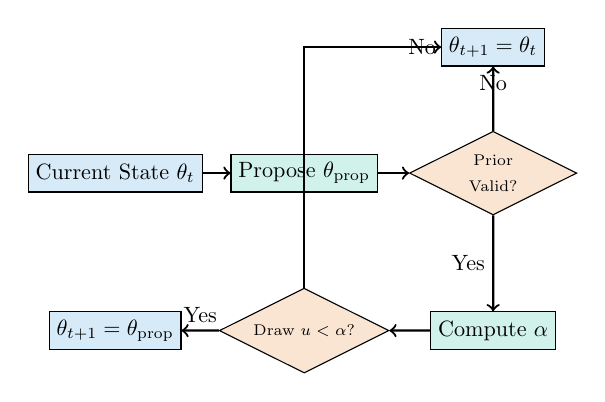
\begin{tikzpicture}[scale=0.8, every node/.style={transform shape}]
    % Nodes
    \node[draw, fill=secondary!20, minimum height=0.6cm] (start) at (0, 0) {Current State $\theta_t$};
    \node[draw, fill=primary!20, minimum height=0.6cm] (prop) at (3, 0) {Propose $\theta_{\text{prop}}$};
    \node[draw, fill=accent!20, diamond, aspect=2, align=center] (prior) at (6, 0) {\scriptsize Prior \\ \scriptsize Valid?};
    \node[draw, fill=primary!20, minimum height=0.6cm] (alpha) at (6, -2.5) {Compute $\alpha$};
    \node[draw, fill=accent!20, diamond, aspect=2, align=center] (check) at (3, -2.5) {\scriptsize Draw $u < \alpha$?};
    
    \node[draw, fill=secondary!20, minimum height=0.6cm] (accept) at (0, -2.5) {$\theta_{t+1} = \theta_{\text{prop}}$};
    \node[draw, fill=secondary!20, minimum height=0.6cm] (reject) at (6, 2.0) {$\theta_{t+1} = \theta_t$};
    
    % Paths
    \draw[->, thick] (start) -- (prop);
    \draw[->, thick] (prop) -- (prior);
    \draw[->, thick] (prior) -- node[left] {Yes} (alpha);
    \draw[->, thick] (prior) -- node[above] {No} (reject);
    \draw[->, thick] (alpha) -- (check);
    \draw[->, thick] (check) -- node[above] {Yes} (accept);
    \draw[->, thick] (check) |- node[right, pos=0.85] {No} (reject);
  \end{tikzpicture}
  \vfill
\end{frame}

% Slide 16: Hand-Worked MCMC Step
\begin{frame}{Hand-Worked MCMC Step}
  Let's walk through a single MCMC parameter step:
  \begin{itemize}
    \item \textbf{Parameter:} Rate parameter $\theta$.
    \item \textbf{Priors:} Flat uniform prior over $[0, 5]$.
    \item \textbf{Current State ($t$):} $\theta_t = 1.0$, with joint numerator score:
      $$P(D \mid \theta_t) P(\theta_t) = 0.040$$
    \item \textbf{Step 1: Propose candidate $\theta_{\text{prop}}$:}
      Draw a step from proposal distribution $\mathcal{N}(1.0, 0.05^2)$, yielding:
      $$\theta_{\text{prop}} = 1.08$$
      Check prior: $1.08 \in [0, 5]$, so the proposal is valid.
    \item \textbf{Step 2: Calculate target score at proposal:}
      $$P(D \mid \theta_{\text{prop}}) P(\theta_{\text{prop}}) = 0.032$$
    \item \textbf{Step 3: Compute acceptance probability $\alpha$:}
      $$\alpha = \min\left(1, \frac{0.032}{0.040}\right) = \min(1, 0.80) = 0.80$$
    \item \textbf{Step 4: Draw random variable $u \sim \mathcal{U}(0, 1)$:}
      \begin{itemize}
        \item If we draw $u = 0.54 \implies 0.54 < 0.80 \implies$ \textbf{Accept:} $\theta_{t+1} = 1.08$.
        \item If we draw $u = 0.87 \implies 0.87 \ge 0.80 \implies$ \textbf{Reject:} $\theta_{t+1} = 1.00$.
      \end{itemize}
  \end{itemize}
\end{frame}

% Module 4 Header
\begin{frame}[plain]
  \vfill
  \centering
  \begin{beamercolorbox}[sep=8pt,center,shadow=true,rounded=true]{palette primary}
    \usebeamerfont{title}\textbf{Module 4: MCMC Diagnostics \& Best Practices}
  \end{beamercolorbox}
  \vfill
\end{frame}

% Slide 18: Trace Plots: Monitoring Convergence
\begin{frame}{Trace Plots: Monitoring Convergence}
  A **Trace Plot** displays the parameter value on the y-axis against the iteration step index on the x-axis. It is the primary diagnostic tool for monitoring chain convergence:
  \begin{itemize}
    \item \textbf{Caterpillar Look:} A healthy, converged MCMC chain looks like a tight, horizontal ``fuzzy caterpillar.'' It oscillates rapidly around a stable mean value.
    \item \textbf{Poor Mixing (Drifting):} If the chain shows long-term trends or slow waves, it has poor mixing. This means the step size is too small or the sampler is stuck in a local region.
    \item \textbf{Tuning Proposal Width ($\sigma$):}
      \begin{itemize}
        \item **Too Small:** Chain accepts almost every step but moves very slowly, failing to explore the parameter space.
        \item **Too Large:** Chain proposes massive jumps into low-probability regions, resulting in almost all steps being rejected (chain gets stuck in horizontal lines).
        \item **Optimal:** Aim for an acceptance rate of $\sim 20\% - 50\%$.
      \end{itemize}
  \end{itemize}
\end{frame}

% Slide 19: Trace Plot Configurations
\begin{frame}{Trace Plot Configurations}
  Below is a conceptual visualization of trace plots under different proposal widths:
  \begin{columns}
    \begin{column}{0.33\textwidth}
      \centering
      \alert{\textbf{Step Size Too Small}}
      \begin{tikzpicture}[scale=0.45]
        \draw[->] (0,0) -- (5,0) node[right] {Iter};
        \draw[->] (0,0) -- (0,5) node[above] {$\theta$};
        \draw[thick, primary] (0,1) -- (1,1.2) -- (2,1.5) -- (3,1.9) -- (4,2.2) -- (5,2.4);
      \end{tikzpicture}
      \scriptsize High acceptance, but slow drift. Fails to explore.
    \end{column}
    \begin{column}{0.33\textwidth}
      \centering
      \alert{\textbf{Step Size Too Large}}
      \begin{tikzpicture}[scale=0.45]
        \draw[->] (0,0) -- (5,0) node[right] {Iter};
        \draw[->] (0,0) -- (0,5) node[above] {$\theta$};
        \draw[thick, accent] (0,2) -- (1,2) -- (2,2) -- (3,2) -- (4,4.2) -- (5,4.2);
      \end{tikzpicture}
      \scriptsize High rejection rate. Long horizontal periods.
    \end{column}
    \begin{column}{0.33\textwidth}
      \centering
      \alert{\textbf{Optimal step size}}
      \begin{tikzpicture}[scale=0.45]
        \draw[->] (0,0) -- (5,0) node[right] {Iter};
        \draw[->] (0,0) -- (0,5) node[above] {$\theta$};
        \draw[thick, secondary] (0,2) -- (0.8,3) -- (1.6,1.8) -- (2.4,2.8) -- (3.2,2.1) -- (4,2.9) -- (5,2);
      \end{tikzpicture}
      \scriptsize Rapid oscillations around the mean. Healthy mixing.
    \end{column}
  \end{columns}
\end{frame}

% Slide 20: Burn-in and Autocorrelation
\begin{frame}{Burn-in and Autocorrelation}
  Before analyzing our MCMC samples, we must apply two preprocessing steps:
  \begin{description}
    \item[1. Burn-In Phase:]
      The starting point $\theta_0$ is often in a low-probability region. The early iterations show a systematic drift as the chain climbs toward the high-probability peak.
      \begin{itemize}
        \item \textbf{Action:} Discard the first $10\% - 20\%$ of the chain (e.g., discard the first 1,000 steps of a 6,000-step chain). This ensures our analyzed samples only come from the converged stationary distribution.
      \end{itemize}
    \item[2. Autocorrelation (Thinning):]
      Because MCMC states depend on preceding steps, adjacent samples are correlated.
      \begin{itemize}
        \item \textbf{Thinning:} We save only every $k$-th sample (e.g., keep every 5th or 10th sample) to reduce correlation and storage size, yielding independent draws from the posterior.
      \end{itemize}
  \end{description}
\end{frame}

% Slide 21: Visualizing Posterior Marginals: Corner Plots
\begin{frame}{Visualizing Posterior Marginals: Corner Plots}
  For multi-parameter models (like Type Ia coefficients $A$ and $B$), we display MCMC results using a \textbf{Corner Plot}:
  \begin{itemize}
    \item \textbf{Diagonal Panels:} 1D histograms showing the marginal posterior distribution for each parameter. The peak represents the best fit, and the width represents the uncertainty.
    \item \textbf{Off-Diagonal Panels:} 2D contour maps or scatter plots showing the joint distribution of parameter pairs.
    \item \textbf{Mapping Degeneracies:}
      If two parameters are uncorrelated, the 2D contour is circular. If they are correlated, the contour is elongated (a degeneracy diagonal).
    \item The MCMC corner plot reveals how parameters trade off against each other, exposing degeneracies that point estimates (MLE) completely hide.
  \end{itemize}
\end{frame}

\end{document}
